\documentclass[12pt,twoside]{article}
\usepackage{jmlda}
\usepackage{lineno}

\usepackage{a4wide}
\usepackage{amsmath, amsfonts, amssymb}
\usepackage[english, russian]{babel}
\usepackage[russian]{babel}
\usepackage{setspace}
\doublespacing
\usepackage[utf8]{inputenc}
\linenumbers
\renewcommand{\baselinestretch}{1.3}
\newcommand{\bX}{\mathbf{X}}
\newcommand{\ba}{\mathbf{a}}
\newcommand{\bx}{\mathbf{x}}
\newcommand{\by}{\mathbf{y}}
\newcommand{\bu}{\mathbf{u}}
\newcommand{\bw}{\mathbf{w}}
\newcommand{\cA}{\mathcal{A}}
\newcommand{\bbB}{\mathbb{B}}
\newcommand{\bbR}{\mathbb{R}}

%\NOREVIEWERNOTES
\title
    [Предсказание качества для процедуры выбора признаков] % Краткое название; не нужно, если полное название влезает в~колонтитул
    {Предсказание качества для процедуры выбора признаков}
\author
    [Аминов Т.В.] % список авторов для колонтитула; не нужен, если основной список влезает в колонтитул
    {Аминов Т.В.} % основной список авторов, выводимый в оглавление
    [Аминов Т.В.] % список авторов, выводимый в заголовок; не нужен, если он не отличается от основного
\thanks
    {Работа выполнена при финансовой поддержке РФФИ, проект \No\,00-00-00000.
   Научный руководитель:  Стрижов~В.\,В.
   Задачу поставил:  Роман~Р.\,В.
    Консультант:  Роман~Р.\,В.}
\email
    {aminov.tv@phystech.edu}
\organization
    {$^1$Московский Физико-технический институт}
\abstract
    {В случае избыточного признакового пространства  предсказатеьная модель машинного обучения является неустойчивой. Для повышения устойчивости модели применяются методы выбора признаков. Задача выбора признаков состоит в поиске решения среди экпоненциального числа возможных решений, поэтому она является NP-задачей. Для решения применяются эвристические, субоптимальные алгоритмы. В данной статье предлагается свести дискретную задачу выбора признаков к задаче непрерывной оптимизации. Строится процедуры предсказания качества модели на тестовой выборке для подмножества признаков. Решение задачи выбора признаков восстанавливается из решения непрерывной задачи. Проводится вычислительный эксперимент, чтобы сравнить результаты предложенного метода с существующими алгоритмами.


\bigskip
\textbf{Ключевые слова}: \emph {Выбор признаков, многомерные пространства, отображение булева куба}.}
\titleEng
    {JMLDA paper example: file jmlda-example.tex}
\authorEng
    {Author~F.\,S.$^1$, CoAuthor~F.\,S.$^2$, Name~F.\,S.$^2$}
\organizationEng
    {$^1$Organization; $^2$Organization}
\abstractEng
    {This document is an example of paper prepared with \LaTeXe\
    typesetting system and style file \texttt{jmlda.sty}.

    \bigskip
    \textbf{Keywords}: \emph{keyword, keyword, more keywords}.}
\begin{document}
\maketitle
%\linenumbers
\section{Введение}
При решении многих задач машинного обучения, таких как классификация и регрессия, исходное пространство признаков оказывается избыточным. Не все признаки коррелируют с целевой переменной, нерелевантные признаки делают модель неустойчивой. Данная работа посвящена проблеме выбора оптимального подмножества признаков. Эта задача является NP-задачей, так как точное решение ищется среди всевозможных $2^n - 1$ вариантов, где n - количество признаков. Поэтому предполагается отыскание приближенного решения.

Задача выбора признаков возникает при  распознавании лиц  ~\cite{inproceedings}. В статье \cite{bertsimas2016} данная проблема в пространствах малой размерности (порядка 1000). За счет огромного прироста вычислительной мощности за последние 20 лет задача выбора признаков может решаться точно за разумное время.В статье ~\cite{cao2018learnable} пердставлена идея построения оптимальной архитектуры нейронной сети . Существующие методы, независимо от того, основаны ли они на обучении с подкреплением \cite{article2} или на эволюционных алгоритмах (EA) \cite{5989810}, выполняют поиск архитектуры в дискретном пространстве, который крайне неэффективен.

 Авторы предлагают простой и эффективный метод автоматического выбора признаков непрерывной оптимизации. Весь алгоритм разбивается на три этапа: (1) енкодер - отображает пространтво подмножества признаков Стрижов пидр в линейное пространство; (2) предиктор - принимает непрерывное представление подмножества признаков  в качестве входных данных и прогнозирует ошибку на тестовой выборке; (3) декодер - отображает непрерывное представление обратно в набор признаков. Существенным отличием нашего метода от уже сущесвтующих состоит в том что размерность булева куба признаков очень велика, а значит для прироста скорости нам придется отображать его в пространство гораздо меньшей размерности.


В качестве показателя эффективности предложенного алгоритма предполагается сравнение с уже существующими : CSO (PSO) \cite{article}, CFS \cite{Gu2018}, QPFS \cite{Rodriguez-Lujan:2010:QPF:1756006.1859900}, на реальных и синтетических данных.


\section{Постановка задачи}
Пусть $\mathbf{X}=[\boldsymbol{\chi}_1,...,\boldsymbol{\chi}_n]\in\mathbb{R}^{m\times n}$ - заданная матрица, где $\boldsymbol{\chi_j}\in\mathbb{R}^m$ - j-ый признак. Пусть  $\by \in \bbR^m$ занчения искомой функции. Множество ~$\cA \subseteq \{1, \dots, n\}$ - индикаторное подмножество признаков. Существует соответствие между множеством ~$\cA$ и двоичными векторами ~$\ba \in \bbB^n$:
\[
	\cA = \{j: a_j = 1\}.
\]
Функция  $f(\bx, \bw, \cA)$ предсказывает $y$ по заданному объекту~$\bx$ и используя только признаки из множества~$\cA$.Данные разбиваются на две части: train $(\bX_{\text{tr}}, \by_{\text{tr}})$ и test $(\bX_{\text{te}}, \by_{\text{te}})$. Чтобы измерить качество модели~$f$, вводится функция функция ошибки~$s(\bw, \bX, \by, \cA)$. Для обучения подбираются наилучшие параметры~$\bw^*$, исходя из условия:
\[
	\bw^* = \argmin_{\bw} s(\bw, \bX_{\text{tr}}, \by_{\text{tr}}, \cA).
\]
 Целью является нахождение такого множества~$\cA$ на котором функция ошибки на тестовой выборке будет минимальна. Предлагается следовать следующему методу. Создается набор данных$\{(\ba_i, s_i)\}_{i=1}^N$. Выбираются $N$ векторов $\ba$ из двоичного куба~$\bbB^n$. Затем оценивается ошибка $s_i$ для каждого набора ~$\ba_i$. Идея в том чтобы отобразить дискретную область~$\bbB^n$ в непрерывную с меньшей размерностью~$h <n$. Таким образом вектор признаков будет обладать непрерывным представлением~$\bu \in \bbR^h$. Это представление создается енкодером~$e(\ba, \bw_e)$. После этого модель~$p(\bu, \bw_p)$ пытается предсказать ошибку на тестовой выборке $s$. Тогда модель принимает вид~$s=p(\bu, \bw_p) = p(e(\ba, \bw_e), \bw_p)$. Возможно использование любой функции потерь для оценки параметров~$\bw_e, \bw_p$. Например это может быть квадратичная функция ошибки
 \[
	L_{error}(\bw_e, \bw_p, \ba, s) = \| p(e(\ba, \bw_e), \bw_p) - s \| ^2 \rightarrow \min_{\bw_e, \bw_p}.
\]
Так же требуется постороить модель обратного отображения вектора~$\ba$ по его непрерывному представлению~$\bu$. Эта модель будет называться декодер~$\sigma(\bu, \bw_{\sigma})$. Вводится функция ошибки отображения - кросс-итропия между начальным вектором~$\ba$ и тем что получаетя на выходе модели декодер~$\sigma$
\[
	L_{rec}(\bw_e, \bw_\sigma, \ba) = \sum_{i=1}^n a_i \log(\sigma_i) + (1 - a_i) \log (1 - \sigma_i) \rightarrow \min_{\bw_e, \bw_\sigma},
\]
где $\sigma_i = \sigma(e(\ba, \bw_e), \bw_{\sigma})_i$.
Общая функция потерь будет линейной комбинацией ошибки предсказания и ошибки отображения
\[
	L = L_{error} + \alpha L_{rec}.
\]
Совокупностью параметров~$\bw_e, \bw_p, \bw_\sigma$ задается наиболее подходящее подмножество признаков. Максимизируется предсказательное качество модели
\[
	\bu^* = \argmax_{\bu} p(\bu, \bw_p).
\]

\begin{figure}[h!]
	\centering
	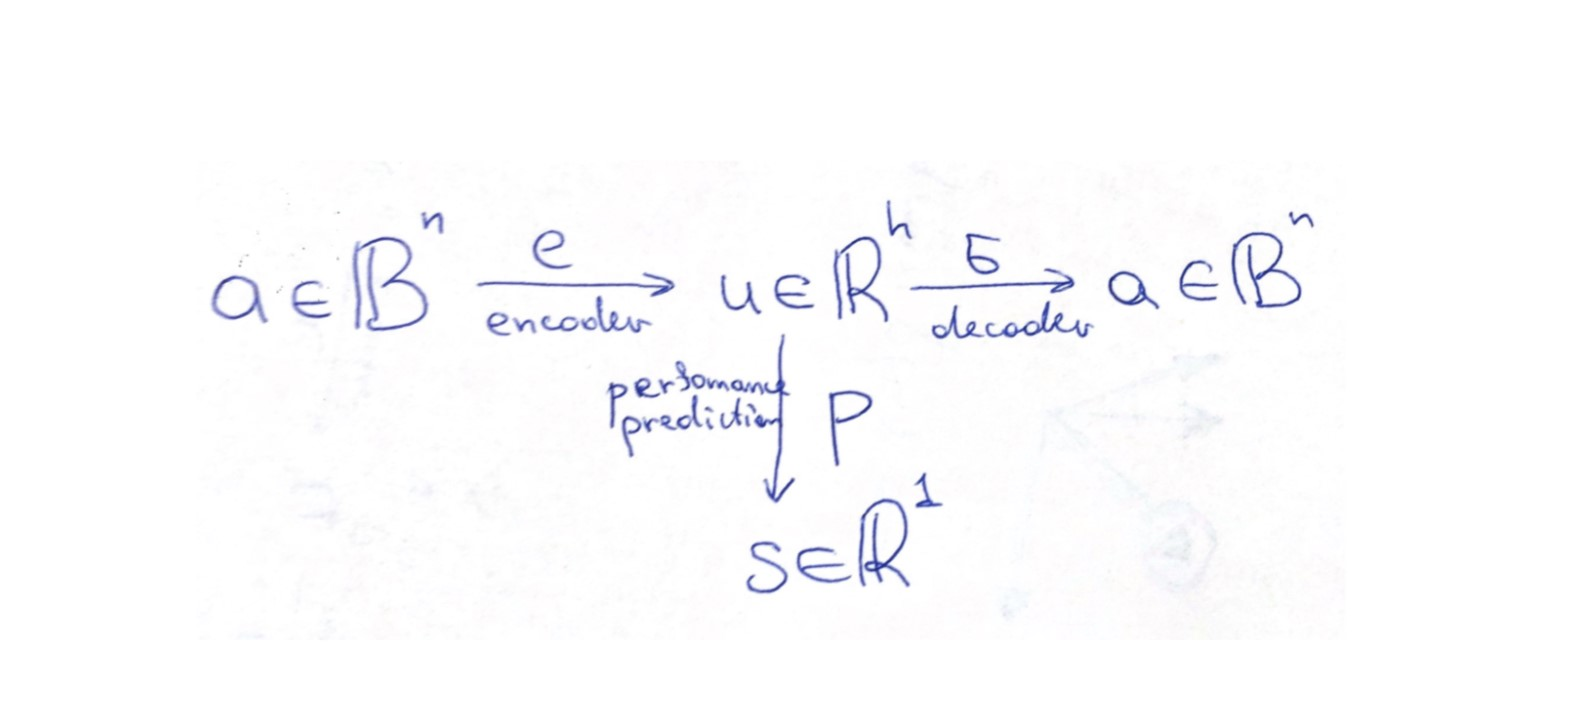
\includegraphics[width=0.8\linewidth]{Jmlda-guides/1.jpg}
\end{figure}






\bibliographystyle{unsrt}
\bibliography{1}
%\begin{thebibliography}{1}

%\bibitem{author09anyscience}
%    \BibAuthor{Author\;N.}
%    \BibTitle{Paper title}~//
%    \BibJournal{10-th Int'l. Conf. on Anyscience}, 2009.  Vol.\,11, No.\,1.  Pp.\,111--122.
%\bibitem{myHandbook}
%    \BibAuthor{Автор\;И.\,О.}
%    Название книги.
%    Город: Издательство, 2009. 314~с.
%\bibitem{author09first-word-of-the-title}
%    \BibAuthor{Автор\;И.\,О.}
%    \BibTitle{Название статьи}~//
%    \BibJournal{Название конференции или сборника},
%    Город:~Изд-во, 2009.  С.\,5--6.
%\bibitem{author-and-co2007}
%    \BibAuthor{Автор\;И.\,О., Соавтор\;И.\,О.}
%    \BibTitle{Название статьи}~//
%    \BibJournal{Название журнала}. 2007. Т.\,38, \No\,5. С.\,54--62.
%\bibitem{bibUsefulUrl}
%    \BibUrl{www.site.ru}~---
%    Название сайта.  2007.
%\bibitem{voron06latex}
%    \BibAuthor{Воронцов~К.\,В.}
%    \LaTeXe\ в~примерах.
%    2006.
%    \BibUrl{http://www.ccas.ru/voron/latex.html}.
%\bibitem{Lvovsky03}
%    \BibAuthor{Львовский~С.\,М.} Набор и вёрстка в пакете~\LaTeX.
%    3-е издание.
%    Москва:~МЦHМО, 2003.  448~с.
%\end{thebibliography}

% Решение Программного Комитета:
%\ACCEPTNOTE
%\AMENDNOTE
%\REJECTNOTE
\end{document}
